\documentclass{TDP003mall}
\usepackage{graphicx}
\graphicspath{ {./images/} }


\newcommand{\version}{Version 1.1}
\author{Hadi Ansari, \url{hadan326@student.liu.se}\\
  Nils Bark, \url{nilba048@student.liu.se}}
  
\title{Installationsmanual}
\date{2020-09-22}
\rhead{Hadi Ansari\\Nils Bark}



\begin{document}
\projectpage
\section{Revisionshistorik}
\begin{table}[!h]
\begin{tabularx}{\linewidth}{|l|X|l|}
\hline
Ver. & Revisionsbeskrivning & Datum \\\hline
1.0 & Första versionen av installationsmanualen & 2020-09-17 \\\hline
1.1 & Komplettering med Flask och Jinja2 & 2020-09-22 \\\hline
\end{tabularx}
\end{table}


\section{Skriva kod}
För att skriva sin kod kan man använda en texteditor som heter Emacs. Ni kan läsa mer om hur man kan installera Emacs på sin linuxbaserade operativsystem här:


\subsection*{Installation av Emacs}

\begin{enumerate}
   \item Öppna terminalen genom att trycka på ALT + Ctrl + t på tangentbordet
   \item Skriv \texttt{sudo apt install emacs}\\
     
\includegraphics[width=60mm]{emacs_install}
   \item Skriv in ditt lösenord
   \item Vänta tills emacs installeras
   \item För att köra emacs after att det installerats kan man skriva \texttt{emacs} i terminalen
   \item För att öppna en fil i emacs så skriver du \texttt{emacs <filnamn>} 
\end{enumerate}

\subsection*{Vanliga fel}
\begin{itemize}
\item Om du vill ha tillgång till terminalfönstret samtidigt som du har öppnat emacs från det fönstret så kan du lösa det genom att lägga till \& på slutet av ditt emacs-kommando
\item Om du har en fil öppen som inte verkar ha färgat texten på rätt sätt, eller inte alls, så beror det troligen på att du har fel (eller inget) filformat på din fil. Åtgärda det och starta sedan om emacs så bör det automatiskt upptäcka formatet
\end{itemize}
\section{Köra och felsöka kod}
För att kunna köra och felsöka sin kod kan man använda sig av följande program.

\subsection*{Skal (terminal)}
Terminalen kan användas som en platform där vi kan köra vår kod och se resultatet av koden. I terminalen kan man även få några felmeddelanden som uppstår när något i koden inte fungerar bra.Ett exempel på detta kan vara om man försöker dela ett tal med noll. Att kontrollera och kunna tolka dessa räknas som en felsökningsmetod som är tillänglig direkt i terminalen.

För att köra din pythonkod i terminalen så skriver du \texttt{python3 <filnamn>} (Glöm inte\texttt{.py}!). Om du vill köra koden i interaktivt läge, som gör att man stannar i pythonmiljön när koden har körts, så får du lägga till \texttt{-i} efter python3. Detta kan vara användbart om man vill t.ex testa specifika delar av sin kod.

Ett tips: Om du har råkat köra ett program som inte kan avslutas, eller som loopar oändligt, så kan du trycka Ctrl-C för att tvinga det att avslutas! 

\subsection*{Pythontutor}
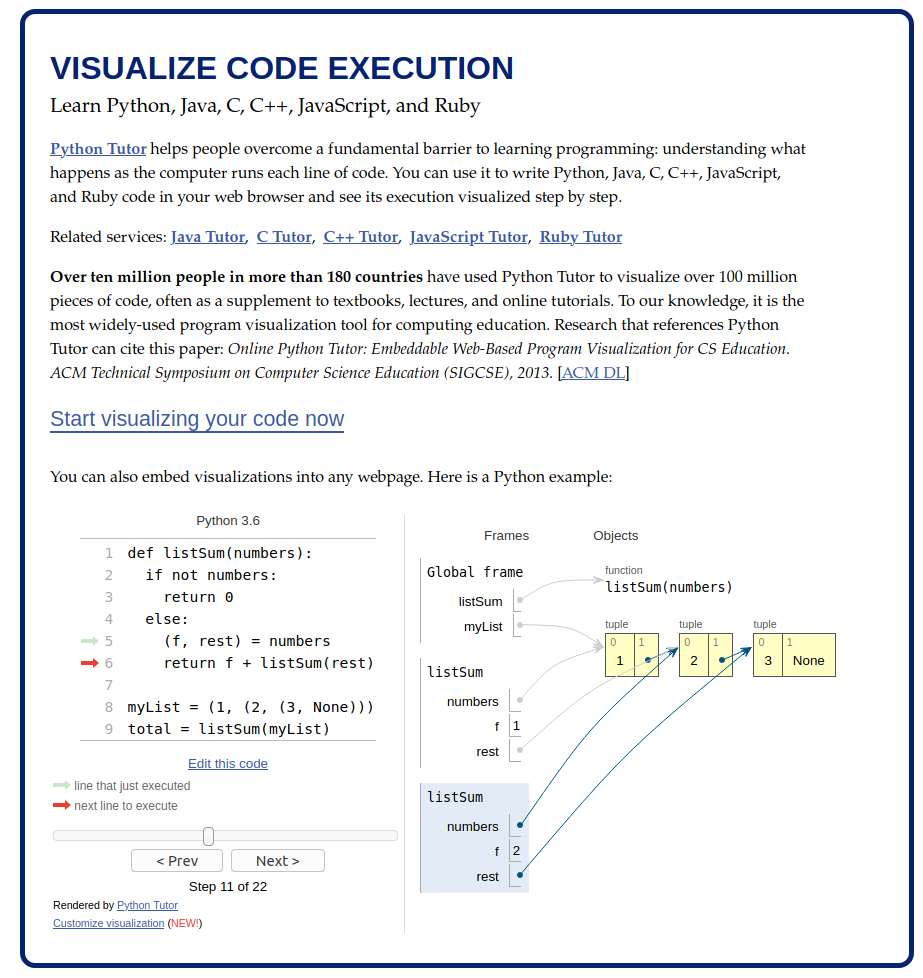
\includegraphics[width=75mm]{pythontutor}

Pythontutor är ett bra verktyg för att kunna köra pythonkod och se steg för steg hur programmet körs. Det kan vara mycket använtbart när man vill felsöka några delar av sin kod som inte fungerar.\\
Pythontutor är en webbsida som man kan få tillgång till genom att skriva adressen \href{http://www.pythontutor.com}{http://www.pythontutor.com} i webbläsaren. Klicka på ``Start vizualising your code now'' För att börja. Sen är det bara att kopiera sin kod och klicka på ``Visulize execution'' för att se hur din kod körs. Se till att välja dem senaste versionen av python, och att du har den senaste versionen av python installerad på ditt system.


\section{Versionhantering}
För att kunna hålla koll på sin utveckling av koden och ha olika versioner av koden sparade på en och samma plats så kan man använda sig av git tillsammans med sitt konto på GitLab. På så sätt kan man ha olika versioner av sin kod sparade vid olika tillfällen och man har möjlighet att gå tillbaka till en specefik version av koden.
\subsection*{Git och Gitlab}
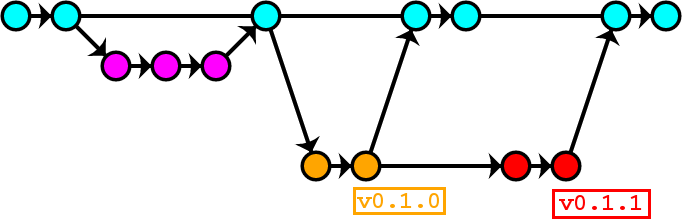
\includegraphics[width=100mm]{git}\\
Så här gör du för att skapa och länka ett GitLab repository till en mapp så att du kan använda dig av Git:
\begin{itemize}

\item Först så går du till GitLabs hemsida (www.gitlab.com) och loggar in.
\item Klicka på ``create project'' och ge det ett namn.
\item Gå in i ``ssh-key'' i inställningarna och kopiera in din dators ssh-nyckel.
\item Du genererar en nyckel genom \texttt{ssh-keygen -t rsa -C ”Gitlab” -b 4096} och hittar nyckeln i ``$\sim$/.ssh/id\_rsa.pub''
\item Navigera till mappen du vill lägga ditt projekt i
\item Kopiera och kör kommandot som börjar med \texttt{git clone} från projektets hemsida
\item Du kan sedan spara dina ändringar lokalt med \texttt{git commit} och sedan spara dem på ditt repository med \texttt{git push}
\item Använd \texttt{git pull} för att hämta hem den senaste versionen av dina filer
\end{itemize}
\subsection*{Vanliga fel}
\begin{itemize}
\item Om du har problem med att köra ditt \texttt{git clone} kommando så beror det troligen på att du inte har länkat rått SSH-nyckel eller att du har fel URL i git clone kommandot. Dubbelkolla att du har tagit hela ssh-nyckeln från textfilen, och att du kopierar hela \texttt{git clone} kommandot som finns på hemsidan till ditt nya och tomma projekt.
\item Om git vill att du väljer att namn/email innan du kan använda commit/push/pull så gör du det med följande två kommandon: \texttt{git config --global user.name "<Ditt namn>"} och \texttt{git config --global user.email "<Din email-adress>"}
\end{itemize}
\section*{Flask och Jinja}
Flask är ett python-ramverk som används inom webbutveckling för flera olika uppgifter. Ett av de packet som följer med Flask är Jinja som bl.a används för att skapa mallar av html-sidor som kan underlätta utvecklingen av en hemsida rejält. T.ex kan man genom att använda Jinja se till att en navbar och footer automatiskt dyker upp på alla sidor, utan att man på egen hand måste kopiera över koden.
\subsection*{Installera Flask (och Jinja)}
Flaskutvecklarna rekommenderar att man skapar ett ``virtual environment'' (vi kommer kalla det för en virtuell miljö) för python för att få bättre kompatibilitet när du jobbar med flask, vilket vi tänker göra här:
\begin{itemize}
\item Skapa först en ny mapp på valfri plats med passande namn
\item Gå in i mappen med \texttt{cd}
\item Skriv \texttt{python3 -m venv venv}
\item Gå igenom installationen
\item Skriv \texttt{. venv/bin/activate} för att aktivera miljön
\item Sedan installerar vi flask med \texttt{pip install Flask}
\item Gå även igenom denna installtionen som vanligt
\item Om allt har gått om det ska så får du detta meddelandet. Notera att Jinja installerades tillsammans med flask:\\
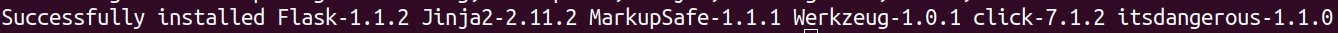
\includegraphics[width=170mm]{Flask2}
\item Testa om allt fungerar som det ska genom att göra en ny .py fil där du skriver \texttt{form flask import Flask}. Se till att den virtuella miljön är aktiverad (Det ska stå ``(venv)'' innan ditt namn i terminalen) och kör sedan filen. Om du inte får några felmeddelanden så fungerar det!

  
\end{itemize}
\subsection*{Vanliga fel}
\begin{itemize}
\item Om du får ett felmeddelande när du försöker skapa din virtuella miljö så är det troligt att du saknas ett pythonpaket. Installera det med \texttt{sudo apt-get install python3-venv} och skriv in ditt lösenord.
\item För att kunna importera och använda flask i dina pythonfiler kommer du behöva aktivera din virtuella miljö innan du kör dem (\texttt{. venv/bin/activate}). För att tillbaka till den vanliga linuxmiljön skriver du bara \texttt{deactivate} i terminalen
\end{itemize}
\end{document}
